\documentclass[10pt,twocolumn,twoside]{osajnl}
%\usepackage[backend=bibtex, defernumbers=true]{biblatex}


\journal{jocn}

% Set the article type for journal submissions. Comment out this line for Optica Open preprint submissions.
\setboolean{shortarticle}{false}
% true = letter / tutorial
% false = research / review article
%\addbibresource{bib.bib}

\title{”Picture Perfect or Ethically Problematic?” \\ Ethical Implications of AI-generated Images on the Example of DALL$\cdot$E 2}

\author[1]{Sofia Kaltwasser}
\author[2]{Manuel Mühlberger}

\affil[1]{University of Potsdam}
\affil[2]{School of Computation, Information and Technology, TU Munich}


%% To be edited by editor
% \dates{Compiled \today}

%% To be edited by editor
%% \doi{\url{http://dx.doi.org/10.1364/XX.XX.XXXXXX}}

\begin{abstract}
	The use of Artificial Intelligence (AI) in image generation has raised ethical questions regarding the role of AI and human artists, ownership and control over generated content, and potential biases. 
	This paper focuses on DALL-E 2, an AI image generation system from OpenAI, to highlight ethical issues that may arise when using AI image generation systems. The paper analyses these issues based on two fundamental moral principles, the Categorical Imperative and Utilitarianism and discusses the current state of regulations and terms of service of providers. The paper also provides an outlook on current research efforts in the European Union for establishing ethical guidelines in AI image generation. The ethical approaches of Kant's categorical imperative and utilitarianism are contrasted to provide a nuanced understanding of the topic and highlight potential ethical dilemmas. The paper further discusses the challenges society may face in the usage of AI-generated images, including the blurred line between inappropriate and acceptable requests. Subsequently, it is presented what is currently being done to ensure ethical handling of AI image generation technology and what further measures can be taken in the future. 
	Overall, this paper emphasizes the importance of critical and ethical analysis in the use of AI image generation technology.
\end{abstract}

\setboolean{displaycopyright}{false} % Do not include copyright or licensing information in submission.

\begin{document}

\maketitle

\section{Introduction}
“I’m fascinated by this imagery. I love it. And it think everyone should see it” is what Jason M. Allen told CNN Business in an interview after winning first prize in the “digital arts/digitally-manipulated photography” category at the Colorado State Fair Fine Arts Competition\cite{JasonMAllenCNN}.
His artwork "Théâtre D’opéra Spatial" (Figure \ref{Theatre}) which he did not draw himself, but was rather generated by an Artificial Intelligence (AI) image generator, raises the question, whether the AI or the human has become the artist and whether Allen is really deserving of the prize.
As these systems become more widespread and accessible, issues such as bias, ownership and control over the generated content will become increasingly relevant, making in-depth critical and ethical analysis vital to ensure that the advantages of this technology are achieved without any detrimental effects. 
This paper will, on the example of DALL-E 2, highlight a select few ethical issues which are likely to come up when using AI image generation systems en masse. 
Thereafter, they will be analyzed based upon two fundamental moral principles, namely, the categorical imperative and utilitarianism. 
It will also shed light on the current state of regulations, or often times lack thereof and juxtapose it with the seemingly arbitrary terms of service that many providers publish. 
Finally, an outlook will be given on current research activity and active efforts in the European Union (EU) for establishing legal liability. 
\begin{figure}[htbp]
	\centering
	\fbox{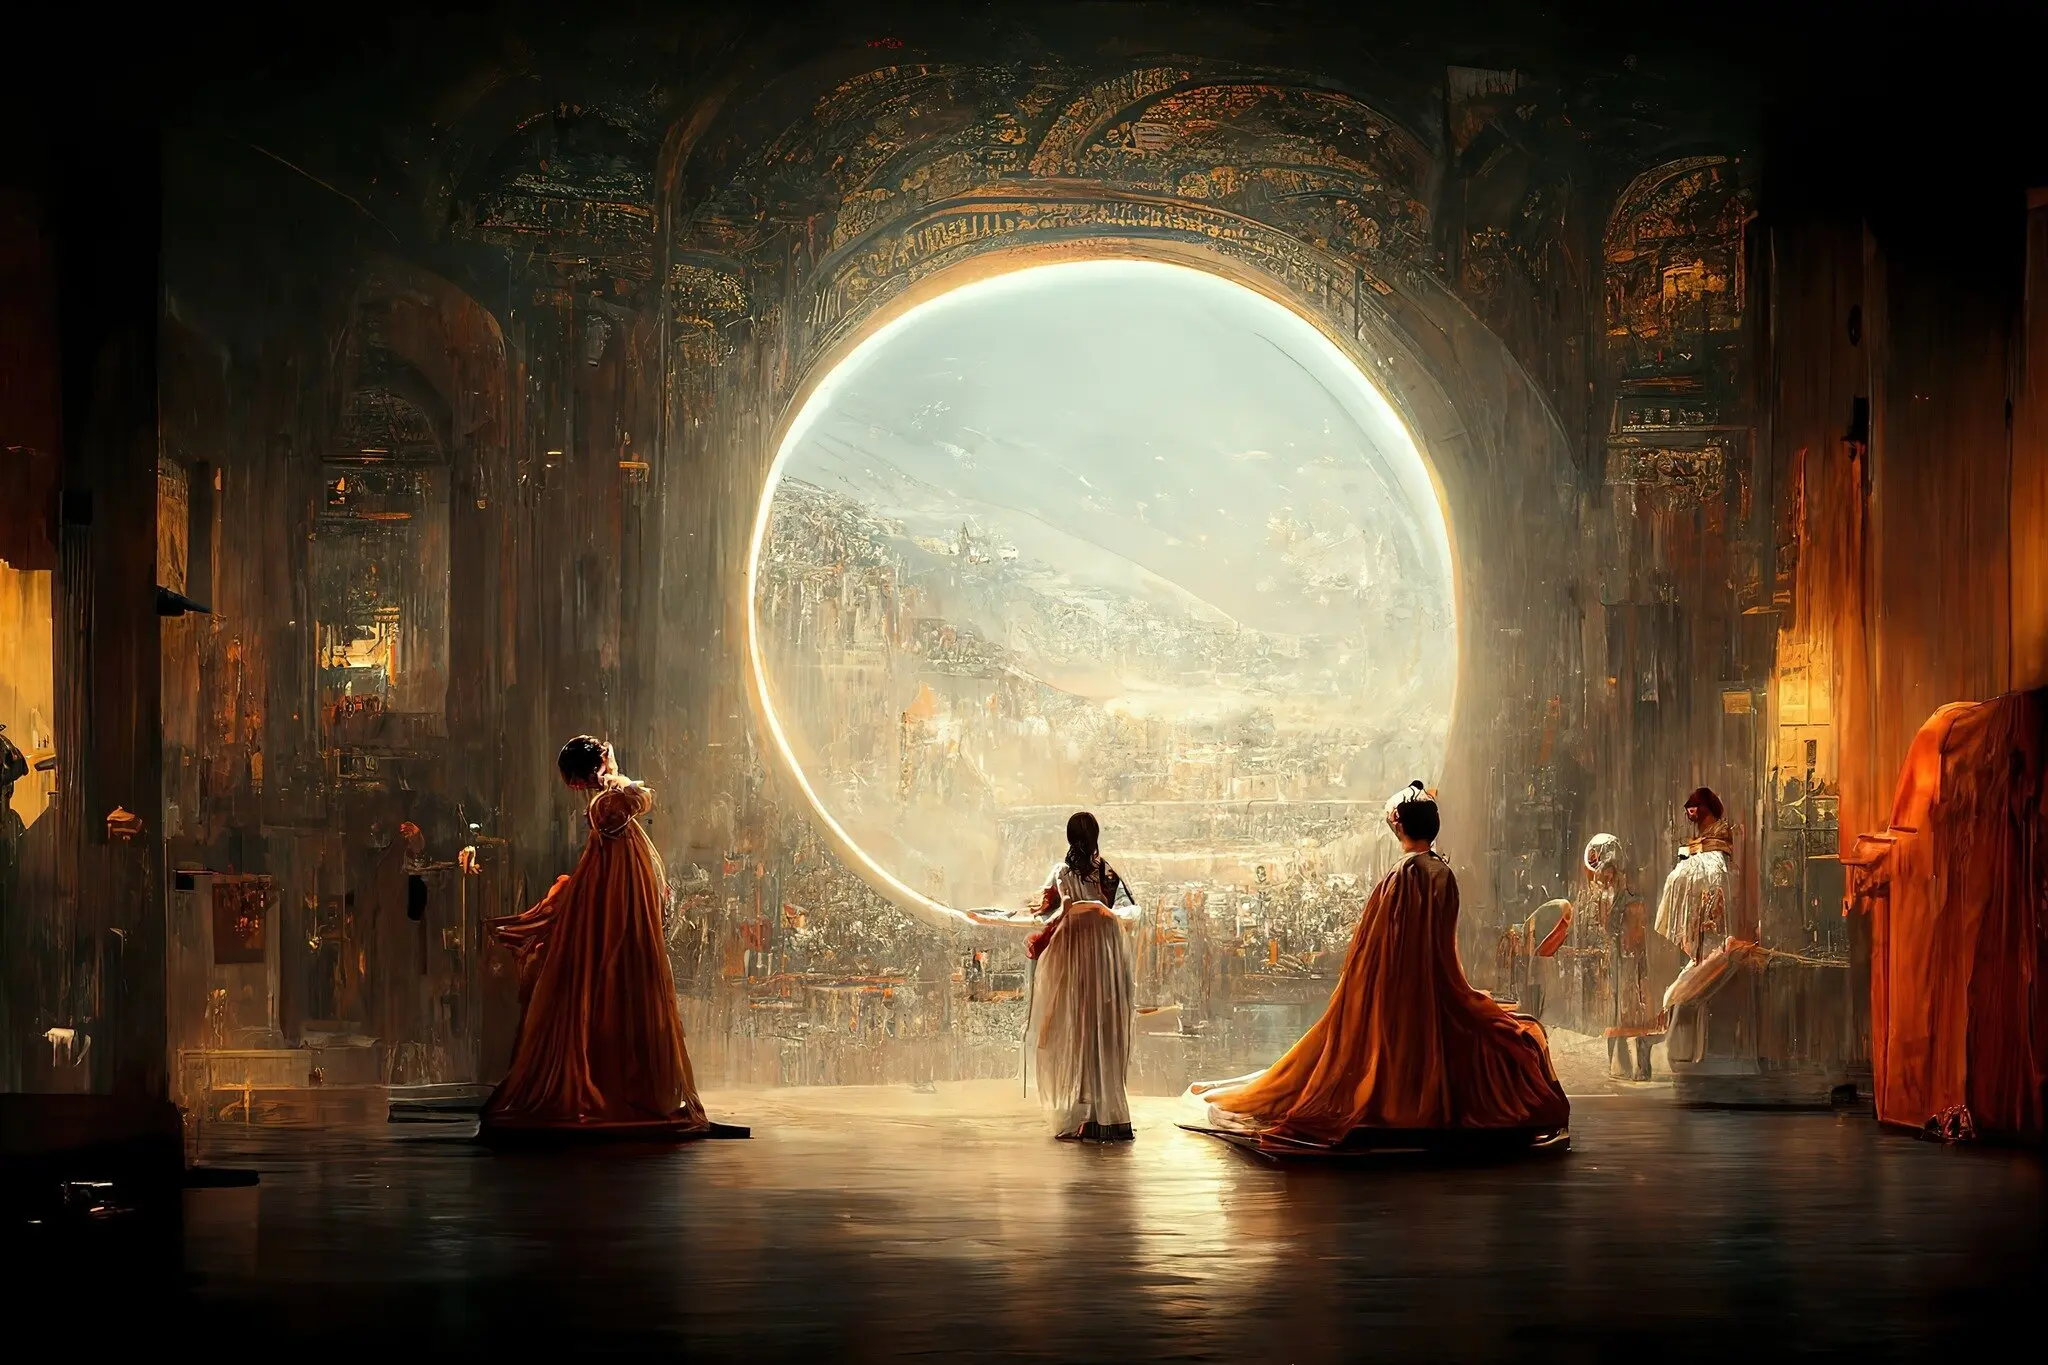
\includegraphics[width=.85\linewidth]{images/ColoradoStateFairWinner.png}}
	\caption{“Théâtre D’opéra Spatial”, Winner of the blue ribbon in the fair’s contest for emerging digital artists by Colorado State Fair’s annual art competition, generated by MidJourneyAi\cite{OperaSpecial}.}
	\label{Theatre}
\end{figure}

\section{Technical Background of DALL-E 2}
In recent years, applications for computer vision and methods for processing images have considerably benefitted from developments made possible by deep learning and AI. 
One of these methods is picture synthesis, which is the act of creating new images and modifying ones that already exist. 
Because of its many useful applications in fields including art creation, image editing, virtual reality, video games, and computer-aided design, image synthesis is a extensive and significant field of research.\\
Text-conditional image models are capable of generating images from text queries and can arrange unrelated objects in a semantically plausible way. They are also called text-to-image models.
One of the most popular examples of such models is Open AI's Dall-E 2 \cite{DallE}.\\ 
%%or images in different styles that can be specified by natural language text queries and has 
DALL-E 2 is a powerful text-to-image synthesis model, released by Open AI in July 2022, capable of extracting the semantic meaning of natural text input and translating it in a zero-shot manner \cite{zeroShot} into high quality images, as can be seen in Figure \ref{exampleTapir}.
Zero-shot learning describes the process of classifying instances during normal usage that were not part of the training set \cite{mfdp}.
In this specific case, this refers to the ability of the user to input text at will that could not have been predicted during training.
It has the potential to be employed in a range of applications, like in creative design. For instance, a digital artist could significantly profit from this technology either by 
finding quick inspiration or by drastically increasing both the speed and the quality of his artwork if he has a certain picture of it in mind.
Overall, it marks a substantial leap in the field of generative models, especially compared to its predecessors DALL-E 1 or DALL-E mini, who where one of the first models that were suitable for the mass\cite{}%TODO: CITATION. 
However, to be able to gauge its possibilities, limitations and draw meaningful ethical conclusions, it is vital to first gain an understanding of its technical backbones.
The following technical background section of this paper will provide an overview of the architecture as well as the training process of DALL-E 2. 


\begin{figure}[htbp]
	\centering
	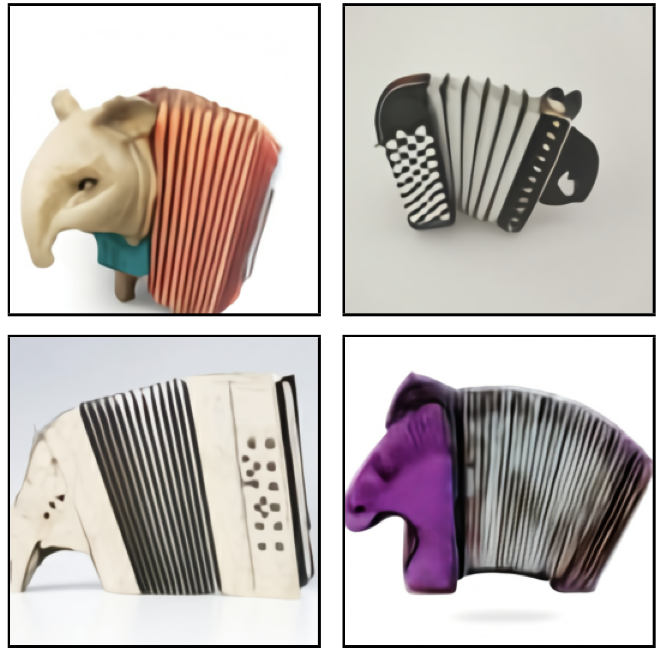
\includegraphics[width=.7\linewidth]{images/DallEExampleTapir.png}
	\caption{Four generated pictures to the text input: "a tapir with the texture of an accordion" \cite{zeroShot}}
	\label{exampleTapir}
\end{figure}

\subsection{Transformer Model}
Vaswani et al. introduced the Transformer model architecture in 2017 \cite{transformer} that has since become the state-of-the-art natural language processing model, whereupon many other models are based.\\
At its core, the transformer is a self-attention-based architecture that operates on sequences of tokens, such as words or subwords. The model contains an encoder and a decoder, each of which consist of a stack of identical layers.\\
Each layer in the transformer is composed of two sub-layers: a self-attention mechanism and a feed-forward network. The self-attention mechanism computes a weighted sum of the input sequence, where the weights are based on the similarity between each token and every other token in the sequence. This allows the model to attend to different parts of the input sequence at different layers, and has been shown to be highly effective at capturing long-range dependencies in language.\\
The feed-forward network applies a set of linear and non-linear transformations to the output of the self-attention mechanism, providing an additional layer of modeling capacity. \\
Apart from that, the transformer features a number of significant modifications in addition to the conventional self-attention mechanism that have proven essential to its success. Multi-head attention, which enables the model to pay attention to various points in the input sequence at once, is one such breakthrough. Another is the use of positional encodings, which provide the model knowledge about the tokens' order in the input sequence.

\subsection{High-level Abstraction of the Text-To-Image Model}
In order to encode the semantic meaning of the corresponding text, DALL-E 2 first processes a textual input description using a transformer-based language model. The multi-stage generative model which creates the final high-resolution image uses the encoded text as input to create an initial low-resolution image that is steadily improved over time, following a diffusion model. The generative model, which creates the image using a combination of transformer- and convolutional-based neural network architectures \cite{T2IReview}. 
%TODO: FINISH SENTENCE?

\begin{figure} [h]
	\centering
	\fbox{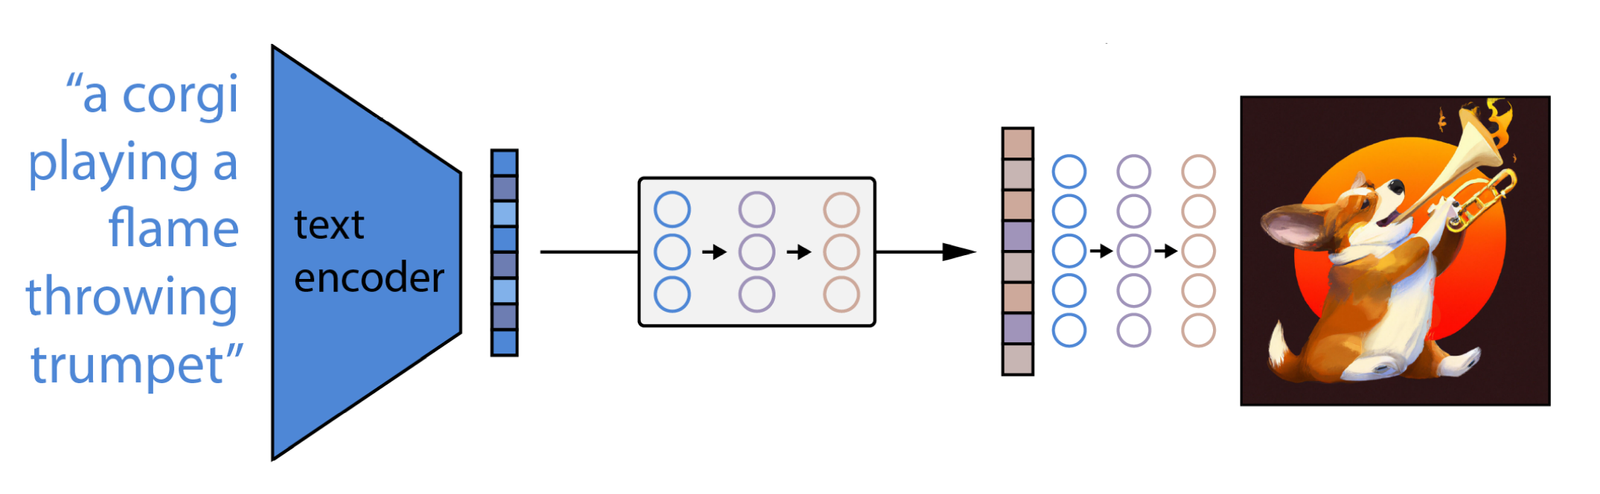
\includegraphics[width = 0.9\linewidth]{images/highLevel.png}}
	\caption{A CLIP text embedding is given to an autoregressive or diffusion algorithm to create an image embedding, which is then used to condition a diffusion decoder to create the final picture in the text-to-image production process.[modified from \cite{CLIP}]}
	%\label{exampleHighLevel}
\end{figure}

\subsection{Training Data}
250 million images and their related textual descriptions were collected from the internet as training data for the first model of DALL-E.\\
It was then trained using a two-stage training procedure \cite{zeroShot}:
\begin{enumerate}
	\item Each 256x256 RGB image was compressed into a 32x32 grid of image tokens with a total of 8192 potential values using a discrete variational autoencoder (dVAE). This results in a factor of 192 reduction in the transformer's context size without noticeably degrading visual quality.
	\item To simulate the joint distribution over the text and picture tokens, an autoregressive transformer is trained using up to 256 BPE-encoded text tokens and 32 x 32 = 1024 image tokens.
\end{enumerate}


\section{Ethical Approaches}
As image synthesis is a relatively young and emerging topic, it can be advantageous to rest the ethical assessment upon applicable philosophical approaches as a known point of reference.
For our evaluation, we have chosen two of the most well-known ethical concepts, namely, the categorial imperative as well as utilitarianism. These two are well suited for the corresponding analysis not only because of their prominence, but also their 
very different points of view.\\
Both will later on be used to perform the ethical analysis and illustrate considerations, potential consequences and the moral principles involved.
By contrasting the categorical imperative with the utilitarianism approach, it is possible to arrive at a more nuanced and informed understanding of the topic, while also highlighting any potential ethical dilemmas that may arise.

\subsection{Kant}
The german philosopher Immanuel Kant (1724--1804) introduced the categorical imperative in his book "Groundwork of the Metaphysic of Morals" in 1785. \\
Kant formulated the categorical imperative as followed: "Act only according to that maxim by which you can at the same time will that it should become a universal law". 
It is a moral principle which states that actions should be taken based on whether they can be willed as a universal law for all individuals in all situations. 
In other words, an action is only morally right if it can be applied to everyone without contradiction.
Although it has been heavily criticized for its abstractness and inflexibility it is still very much relevant today and has a significant role to play in modern ethics and can be applied to a wide range of topics. %TODO: QUELLE!


\subsection{Utilitarianism}
Utilitarianism is an ethical theory based on ideas of Jeremy Bentham (1748--1832) and John Stuart Mill (1806--1873) and builds upon on the so-called Greatest Happiness Principle.%\cite{Cf.}.
It is a form of consequentialism and hence delineates right from wrong by focusing solely on the outcomes of a particular action. 
"[A]ctions are right in proportion as they tend to promote happiness, wrong as they tend to produce the reverse of happiness"\cite{utilitarianism}, whereas happiness can be understood as intended pleasure and the absence of pain.
Furthermore, it is not about an individual's own greatest happiness, but about the greatest happiness of all individuals combined\cite{utilitarianism}. 
The theory assumes that the most ethical decision is the one that produces the greatest utility for the greatest number of people.
Therefore, it is possible that great harm to a minority is disregarded in favor of a small benefit to a majority (greatest happiness of all individuals combined).
\\
%Due to the way, it takes advantages and costs into account, 
Moreover, it is also the method of moral reasoning that is most frequently applied in business \cite{EthicsUnwrapped} and is the moral system that is most known to defend using force or going to war. \\
However, utilitarian ethical decision-making also has its limits. Often times the exact consequences of an action are not certainly predictable.


\subsection{An Ethical Example - The Trolley Problem}
The well-known ethical dilemma called "The Trolley Problem" is well suited to emphasize these two concepts' differences in ethical assessment. 
The Trolley Problem describes a fictional scenario, a thought experiment, in which a spectator has the choice to rescue five people who are in danger of being hit by a trolley, by diverting the trolley to kill just one other person. 
A utilitarianist would pull the lever and save the five people, since the utility of saving five lives is higher than the one of only saving one. A Kantist on the other hand
does not value consequences and would therefore not pull the lever, as one should not kill one person to save five other lives since killing another individual will also be immoral in Kantian ethics. 


\section{What Ethical Challenges exist?}
Like with any emerging technology, there do not only come possibilities, but also challenges society has to face in its usage.
The ability to synthesize images from a text input by the user gives great potential for misuse. \\
Companies like Open AI try to train their models to decline inappropriate requests, but the line between inappropriate and acceptable requests is blurred and difficult to pin down precisely. 
Besides that, there are also models like Stable Diffusion \cite{StableDiffusion} available, which, as of now, cannot be regulated in a meaningful way. 
This is the case because it is open-source in nature and anybody can modify or distribute the source code, so that there does not exist a single point of liability.
In this section a handful of problems will be outlined that are later on to be analysed with the help of the aforementioned moral principles.

\subsection{Social Biases and Stereotypes}
Text-to-image generative models have been shown to have varying amounts of biases, especially gender and skin tone biases. 
When the model is prompted with seemingly neutral phrases (such as "a photo of a nurse") that include no indications to, for example, skin tone or gender, it is nevertheless likely to produce images that are biased towards a certain complexion.
In the above example the generative model is heavily biased towards generating images of white women, as can be seen in Figure \ref{PhotoOfANurse}. 
More specifically, in this example, Stable Diffusion, a competitor to DALLE-2, overwhelmingly generates images of white women, the often times associated stereotype to this profession.
In particular, a study by scientists from UNC Chapel Hill where these biases were measured by the variance of the gender/skin tone distribution through both automated and human evaluation
was able to determine a clear relationship between the training data - labeled images - and the skin tone/ gender biases\cite{DallEval}. 
Although the example here is of Stable Diffusion, the same phenomenon can be observed for DALLE-2 \cite{DalleSocialBias} where the stereotypes are sometimes even more distinctive. 
For instance, DALLE-2 on average portrays 27\% less women in a profession than the United States' Bureau of Labor Statistics (BLS). The BLS registers and collects the actual 
amount of people employed and details other labor market statistics, such as the gender distribution across professions. Compared to DALLE-2 Stable Diffusion produces only 9\% less images of women than the actual 
reported figure\cite{stablebias}. 

\begin{figure}[htbp]
	\centering
	\fbox{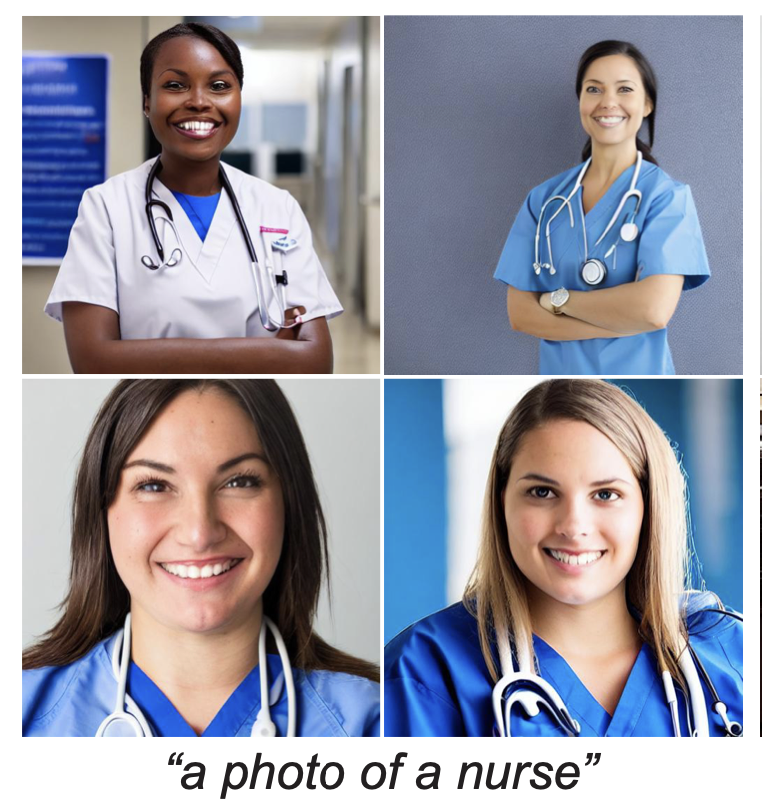
\includegraphics[width = 0.6\linewidth]{images/PhotoOfNurse.png}}
	\caption{Example of social bias: with the prompt "a photo of a nurse". Modified from \cite{DallEval}.}
	\label{PhotoOfANurse}
\end{figure}


\subsection{Portrayal of racism, porn, illegal actions}
Another downside of DALLE-2 which should not be left out are the negative consequences that center around one's ability to generate any image at will. 
Therefore, it is inevitable, that malicious actors will eventually generate harmful, forbidden or illegal imagery. 
Although AI model companies try to restrict what can be generated from a prompt, as discussed in \ref{section:6}, there will always be workarounds to circumvent these safety-restrictions.
Consequently, it is possible to generate images that for instance could portray a child smoking which to our western mindset represents an illegal action. 
Apart from that, other contents harmful to society could be of pornographic or racist nature and may even be considered a felony such as generating child pornography. 


\subsection{Deception, Political Propaganda and Extremism}
One of the biggest dangers encompassing AI generated images are politically motivated and abusive contents like so-called deepfakes\footnote[1]{TEST}. 
Especially in the current times of social media, where uploaded contents go viral\footnote[2]{"Used to describe something that quickly becomes very popular or well known by being published on the internet [...]"\cite{viral}.} 
within minutes or hours and where there does not exist a dedicated supervisory authority, the danger of FakeNews being spread across country or even the whole globe is tremendously large and can bring about severe damage. \\ 
For example on March 23rd, 2023, Donald Trump, the former president of the United States, had images circulate of him 
were he allegedly resisted arrest and was tackled to the ground by the police. This image was uploaded on Twitter and has been viewed over five million times in a few days. Despite the fact that the original creator 
only ever intended for it to be a joke, the AI-generated picture has still drawn a lot of attention within this short timeframe\cite{trump}. In this case, the creator clarified that the image 
was not real and that no harm was intended, however in other scenarios where indeed malicious intentions are present, differentiating a fake image from a real one may be problematic and may also lead to severe reputation damage.
\\
Apart from that, another threat to the wellbeing of society is extremism. With the innovation of AI comes the opportunity for easily accessible tools that allow
for quick content creation without requiring any specific skill set. This way, appealing or persuasive extremist media or similar can rapidly be generated
and brought into circulation, which enables extremists to produce more content of equal quality with less effort than before\cite{AIPropaganda}.
Especially concerning is the fact, that many of the often times preferred mediums can be generated in an (almost) fully autonomous manner through the combination of multiple AI systems.
It may, for instance, be possible to create modifications for a video game within minutes using only the help of an assortment of AI tools.
Researchers from the Global Network on Extremism and Technology were able to generate code to modify a Python video game as well as plotlines for a potential game story with the help of ChatGPT. 
3D assets for guns as well as video game cover art were created using Scenario and MidJourneyAI\footnote[4]{Scenario is an AI used to create computer-generated game assets. MidJourneyAI
is an AI tool to generate images much like DALLE-2 or Stable Diffusion.}. This case demonstrates once more with what ease it is possible to create harmful content without any real effort \cite{AIPropaganda}. 

\begin{figure}[htbp]
	\centering
	\fbox{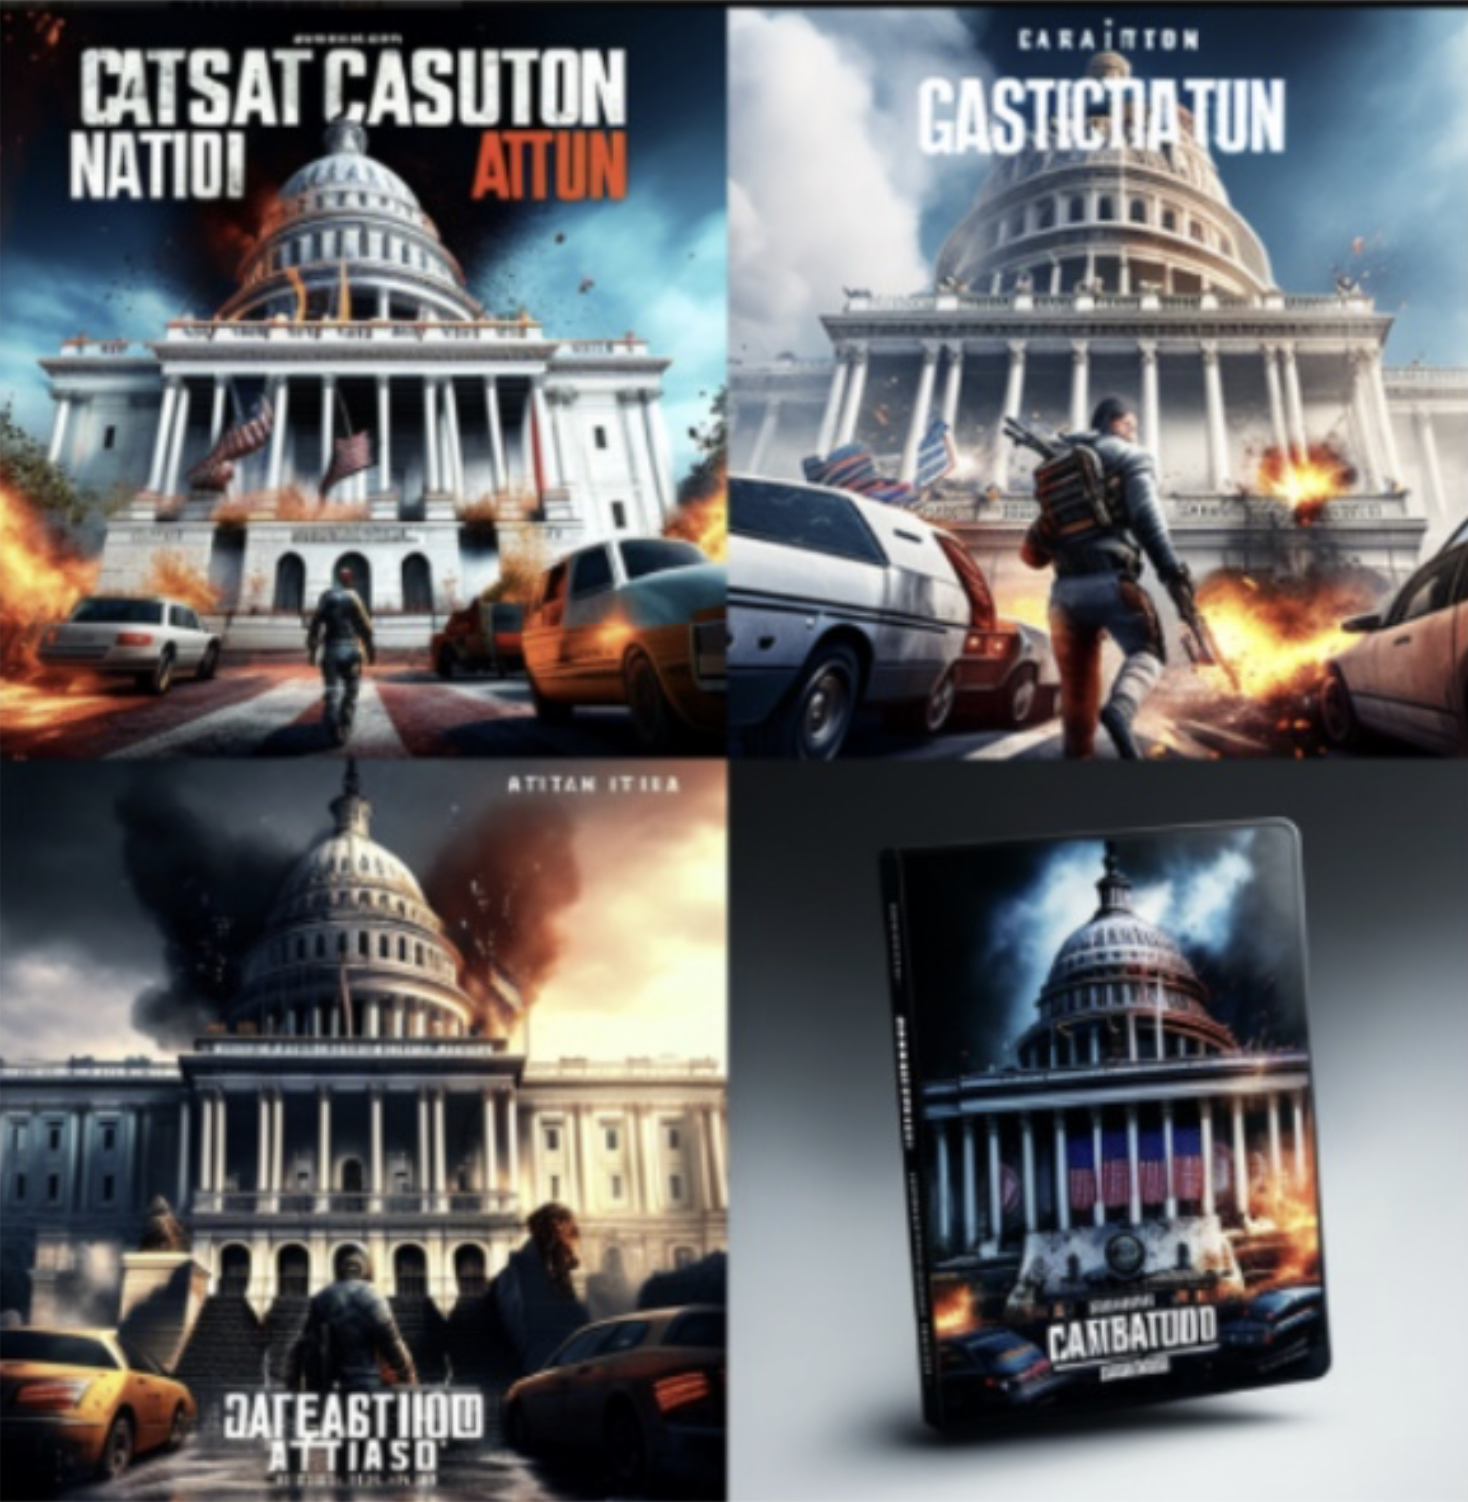
\includegraphics[width = 0.6\linewidth]{images/GameCoverArtCapitolInsurrection.png}}
	\caption{Jan 6. U.S. Capitol insurrection video game art generated by MidJourneyAI, modified from \cite{AIPropaganda}.}
	\label{capitol}
\end{figure}

\section{Ethical Examination}
Taking into account all of the aforementioned aspects, it is significantly relevant to examine whether the use of image generating models in malicious edge cases is ethically justifiable, when considering the extensive consequences
that they may entail. In the first place, the question whether generating political propaganda is morally justifiable will be discussed. 
\\
%Is it ethically acceptable to generate pictures of others without their permission or propaganda material that influences many people after publication. What about pornography or even child pornography?\\
%In the following section, we address the question of which ethical decision-making justifies which application of image generation models.

\subsection{Case A - Political Propaganda}
For assessing the usage of AI to supplement political propaganda according to Kantian Ethics, it has to be "test[ed] whether you could will it to be permissible (under the moral law) for everyone to act on the maxim"\cite{kant}.
Following Kant's definition of a lie, being "an intentionally untruthful statement that is contrary to duty [...]"\cite{kant}, political propaganda can in most cases be clearly categorized as a such.
Propaganda always builds upon bad intentions and aims to influence public thinking towards a malicious goal or a justification thereof. A common example could be convincing the public
of the necessity of a war for the sake of the population's safety. Under this theory, propaganda cannot be assessed as permissible since it would do harm to every individual's rights.
The intentionally wrong information provided through propaganda could possibly impact any individual's opinion and will inevitably cause the formation of opinions based 
upon false information. As a consequence, one would not will propaganda to be permissible as it would compromise truthful shaping of public opinion. 
Apart from that, a lie is by its nature wrong as it is contrary to duty \cite{kant} and %p.240
since propaganda satisfies Kant's definition of a lie, it can be concluded that propaganda is wrong following Kantian Ethics. 
As AI image generation systems like DALLE-2 are easily accessible and usable in nature, they provide quick aid in the production of propaganda which can subsequently be spread across a plentitude
of distribution channels, see Figure \ref{capitol} and \cite{trump} for an example. Due to the fact, that these AI models may facilitate such actions, it is not morally justifiable to use these image generation systems for
political propaganda with respect to Kantian Ethics.
\\ % UTILITARIANISM
For assessing the usage of AI to supplement political propaganda according to Utilitarianism, it has to be identified whether using these systems for this use case creates the greatest utility
for the greatest number of people. First of all, it has to be annotated, that the ethical evaluation according to this theory heavily depends on the distribution of people being pro-propaganda and 
contra-propaganda. Therefore, the evaluation is split into two parts - one supposing the pro-propaganda party to be in the minority and one supposing it to be in the majority.
\\
%PRO-PROPAGANDA MINORITY
Beginning with the first case, the pro-propaganda party represents the minority of people which implies that the majority of people is contra-propaganda. In this case,
allowing for the usage of image generation models to facilitate the creation and propagation of propaganda is beneficial for the pro-propaganda site and therefore creates great utility for this part of the population.
However, for the other part of the population being provided with intentionally false information through propaganda does the contrary since it will inevitably lead to the formation of opinions based on 
invalid information and would hence compromise truthful shaping of public opinion, as mentioned before. 
As the majority of people would be negatively affected by these actions, the greatest utility for this group of people would rather lie in avoiding such methods as it causes harm to the greatest amount of people. 
Consequently, it is not ethically justifiable to use the image generation systems for political propaganda with respect to this scenario and Utilitarianism.
\\
Referring to the second case in which the pro-propaganda party represents the majority of people, the ethical assessment looks very different.
Under this assumption, the usage of image generation models would enable the pro-propaganda party to produce propaganda images in a quick, yet reliable and convenient fashion to afterwards 
propagate them via various distribution channels. In this scenario, the usage of such systems would generate the greatest utility for the greatest amount of people, since the pro-propaganda party 
forms the majority. The negative outcome for the minority is neglectable here as this group of people does not equal to the greatest amount of people. Consequently, it is ethically justifiable to use the 
image generation systems for political propaganda with respect to this scenario and Utilitarianism. 
However, this only applies to the assumption, that other populations like neighboring states or the whole world's population are excluded from the consideration. 

\subsection{Case B - Social Biases and Stereotypes}
%Ist es OK, dass in Dalle gewisse Personengruppen überproportional vertreten sind und Stereotypen verstärkt werden? 
%Durch die Unterrepräsentation von Minderheiten in den Trainingsdaten
For assessing whether it is morally justifiable that AI image generation models such as DALL-E 2 overrepresent certain groups of persons and thereby amplify stereotypes, it is necessary to 
identify whether the Categorial Imperative by Kant is satisfied or not. Therefore, the leading principle, that one should act in a way that it could also be a universal law \cite{kant}, has to be fulfilled. 
According to Kant and his ethics "every human being has equal dignity (or absolute worth)" \cite{kant}. Consequently, any human being is worth as much as any other and discrimination is hence always immoral. 
\\
Because any AI will inevitably mirror inequalities originating from its training set, so the data it learned from, these inequalities will also be reflected in images generated by the AI. 
Hence, in case of current image generation models, that are based on often times skewed training data, which do not always depict reality reliably, equality of all human beings is not guaranteed.
By representing, for instance, specific ethnicities stronger than others, it is suggested that human beings differ in their worth in terms of social class or relevance. 
Under this condition, it is not justifiable that AI image generation models overrepresent certain groups of persons and thereby amplify stereotypes, with respect to Kantian Ethics.
\\
For assessing whether it is morally justifiable that AI image generation models such as DALL-E 2 overrepresent certain groups of persons and thereby amplify stereotypes, under Utilitarianism,
it is necessary to evaluate the scenario of greatest utility for the greatest amount of people. Therefore, in our case, the utility of the majority of people is to be weighed up against the utility of the underrepresented 
minority. To do that, the severity of the harm done to the minority has to be weighed up against the utility resulting from the overrepresentation for the majority. Generally speaking, 
the overrepresentation of certain ethnicities does not generate any significant added value, whereas the effect of the underrepresentation of the minority is to be evaluated as more severe in terms of the harm 
it does to the minority. Due to the underrepresentation, certain groups of people may feel less like they belong to a specific social group or profession and may become isolated from the society. This can cause
severe societal damage as those people may therefore wrongly decide to, for instance, not pursue a profession they would be able to and would excel in, simply because public perception suggests them,
that they are not well-suited for this specific profession, by such skewness in data. This, in turn, can in theory cause worse staff allocation for a given position as some of the more capable persons,
who do not identify themselves as well with the role, choose to not pursue this position. As a consequence, this can lead to a significant decline of the overall societal utility since positions 
may not be taken by the most competent laborer. Due to the tremendously fast growing popularity and importance of AI and AI generated contents, it will be inevitable that any type of results generated 
by AI will be seen by a continuously growing amount of people. The contents generated by those will, unconsciously as well as consciously, impact the perceptions and lives of the whole of society and will therefore
influence decisions they make in the future.  
However, this evaluation has to be taken with a grain of salt, since DALLE-2 is an AI model used globally, so a wholesale statement cannot be determined. This is the case 
since the perceived utility of the majority and minority are subjective and may vary based on different variables, such as ethnic or social group. Apart from that,
the perception may also vary from country to country as every population's and country's situation is a different and individual one. 
For instance, if the result of the prompt shown in Figure \ref{PhotoOfANurse} was shown to a German citizen, the probability that he would think of it as a good representation of a nurse would be 
fairly large, whereas in South Africa the opposite would be the case. Therefore, it highly depends on the perspective that is adopted.
All in all, under the aforementioned conditions, it is hard to formulate a generalized judgement as there are many variables to consider, when ethically assessing with the help of the utilitarian approach.
However, with the perspective adopted above, the harm that is done to the minority is to be assessed as being more severe than the utility gained for the other part of society. Hence, under Utilitarianism,
it is not morally justifiable that AI image generation models overrepresent certain groups and underrepresent others.  

\section{What is currently being done?}
\label{section:6}
With all dangers and challenges AI image generation models entail, the companies behind those systems have already identified potential harm sources and have taken measures to counteract misuse.
In their Terms of Service (TOS), OpenAI states, that DALLE-2's capacity to produce violent, hateful, or pornographic images is constrained. 
For this to work, data filtering was applied to the images depicting violence and sexual content so that data was filtered out of the dataset before training DALLE-2.
More precisely, OpenAI developed a classifier that detects harmful images: in a first step the classifier was trained on image-text pairs labeled by humans, to define categories 
of prohibited content. In the consecutive step, more pictures for each of those categories were gathered and trained on to increase precision. Finally, the classifier was run on the entire 
training data set of DALLE-2, whereas its sensitivity was set in such a manner that it would prefer sorting out data instead of keeping potentially unsafe data. 
To guarantee and validate the functioning of the applied data filters, two so-called GLIDE\footnote[5]{ERKLÄREN} models were trained, one on the dataset before filtering and one on the dataset after.
It was shown that "the filtered model generally produced less explicit or graphic content in response to requests for this kind of content"\cite{openaifilters}. 
\begin{figure}[htbp]
	\centering
	\fbox{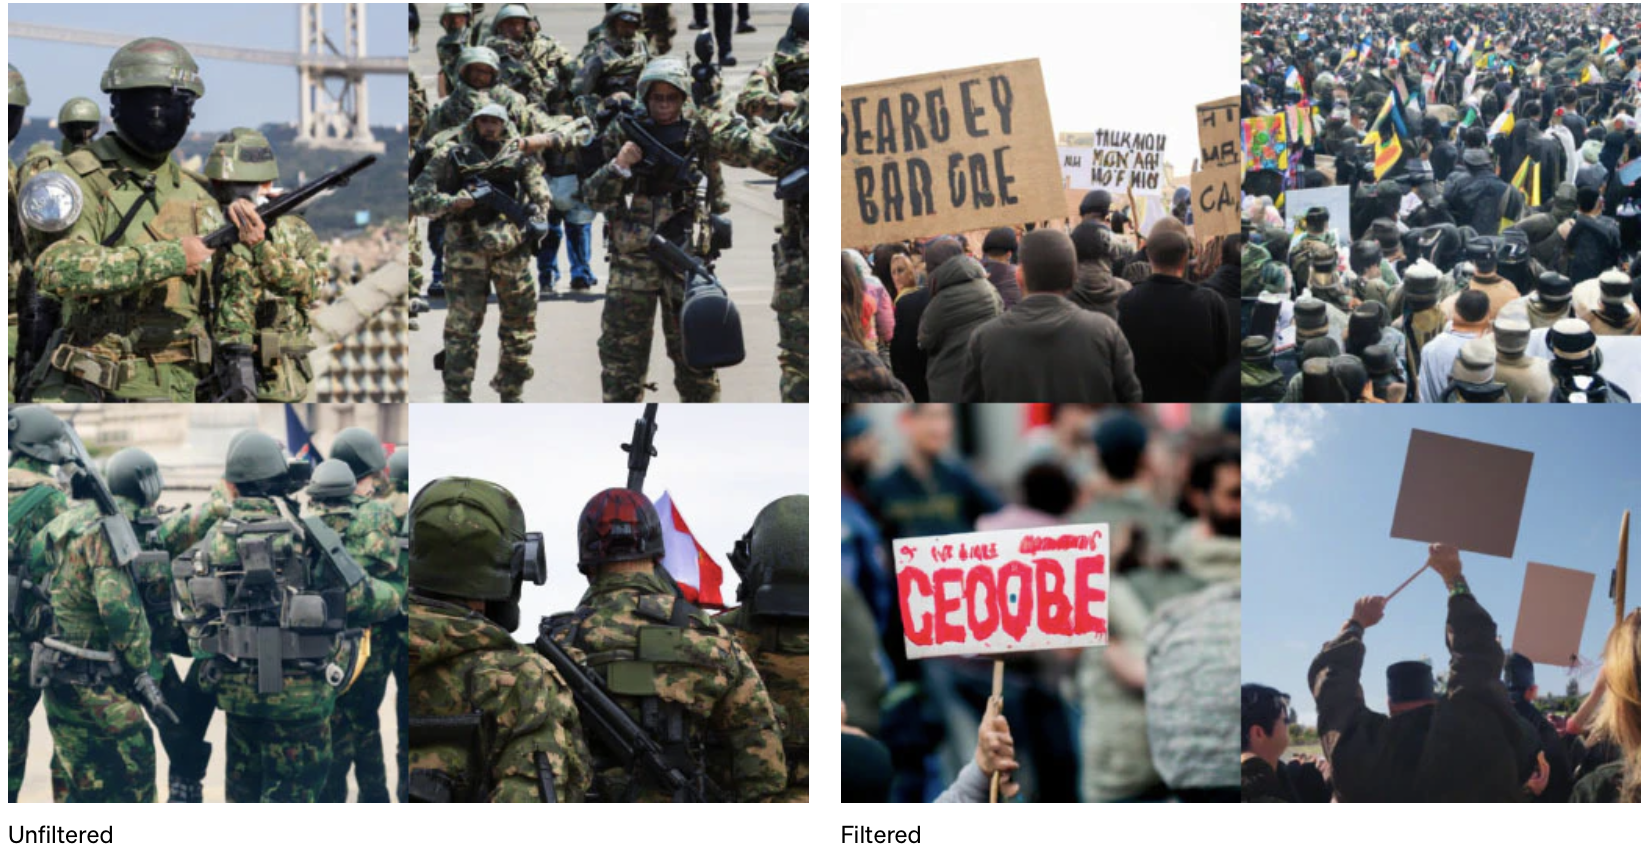
\includegraphics[width = 1.0\linewidth]{images/filters.png}}
	\caption{Generations for the prompt "military protest" from the unfiltered model (left) and the filtered model (right). 
	It is noticeable, that the filtered model almost never produced images of guns \cite{openaifilters}.}
	\label{filters}
\end{figure}
\\
Another issue OpenAI is working on is social bias. To quantify the amount of bias contained within the data set used for training DALLE-2, a keyword search was conducted 
which revealed that, especially after applying the filter against harmful images, some groups of keywords were overrepresented whereas others were underrepresented. 
To fix this problem, the underrepresented images were weighted more to make up for the difference in frequency \cite{openaifilters}. 
\\
Apart from that, OpenAI also blocks image uploads as well as image generation that contain faces of public figures, especially politicians and celebrities. 
This is done to avoid the misuse of DALLE-2 to create deceptive or harmful images \cite{openaiimage}. 
\\
Lastly, every image generated using DALLE-2 includes a small watermark to distinguish it from a real world image \cite{openaicp}. 
However, it is questionable to what extent the watermark actually serves as a way to definitively mark the content since it can easily be removed.

-Simple Watermark\\
-strict regulation in China\\
-no regulation in the west (eu ai law proposal?)\\

\subsection{Data Labeling}
A TIME's investigation revealed that OpenAI used outsourced Kenyan laborers to label text snippets of violence, hate speech, and sexual abuse to generate training data for their ChatGPT’s (Chat Generative Pre-trained Transformer) predecessor, GPT-3 (Generative Pre-trained Transformer 3) that uses deep learning techniques to generate human-like text and engage in conversational interactions and payed them less than 2 US \$ per hour \cite{KenyaExclusive}. The continuous exposure of people to this content is very likely to cause psychological consequences.

\section{What could be done?}
\subsubsection*{Limit Training Data}
To hinder text-to-image models from generating inappropriate images the training data can be limited but therefore data that is inappropriate from a commonsense morality  point of view must be labeled as such. But overall quality could degrade depending on how many and which training data are left out.\\
Other models can be trained to recognize immoral pictures and texts but human supervising is also needed.
In order to prevent people from constantly being confronted with textual or pictorial images of violence, companies could join forces and make their already labeled data available to others and use already existing databases like the Socio-Moral Image Database \cite{Database}.



\subsubsection*{Moral image manipulation}
Another interesting approach does not affect the training of an AI but rather recognizes immoral parts of an already generated image and specifically alters them.
Park et al. introduced  %\cite{MoralEditing} 
a model recognizing visual commonsense immorality of a given picture, localizes the immoral parts of the image and manipulates it into a morally-qualifying alternative, see figure %\ref{moralEditing}.

\begin{figure}[htbp]
		\centering
		\fbox{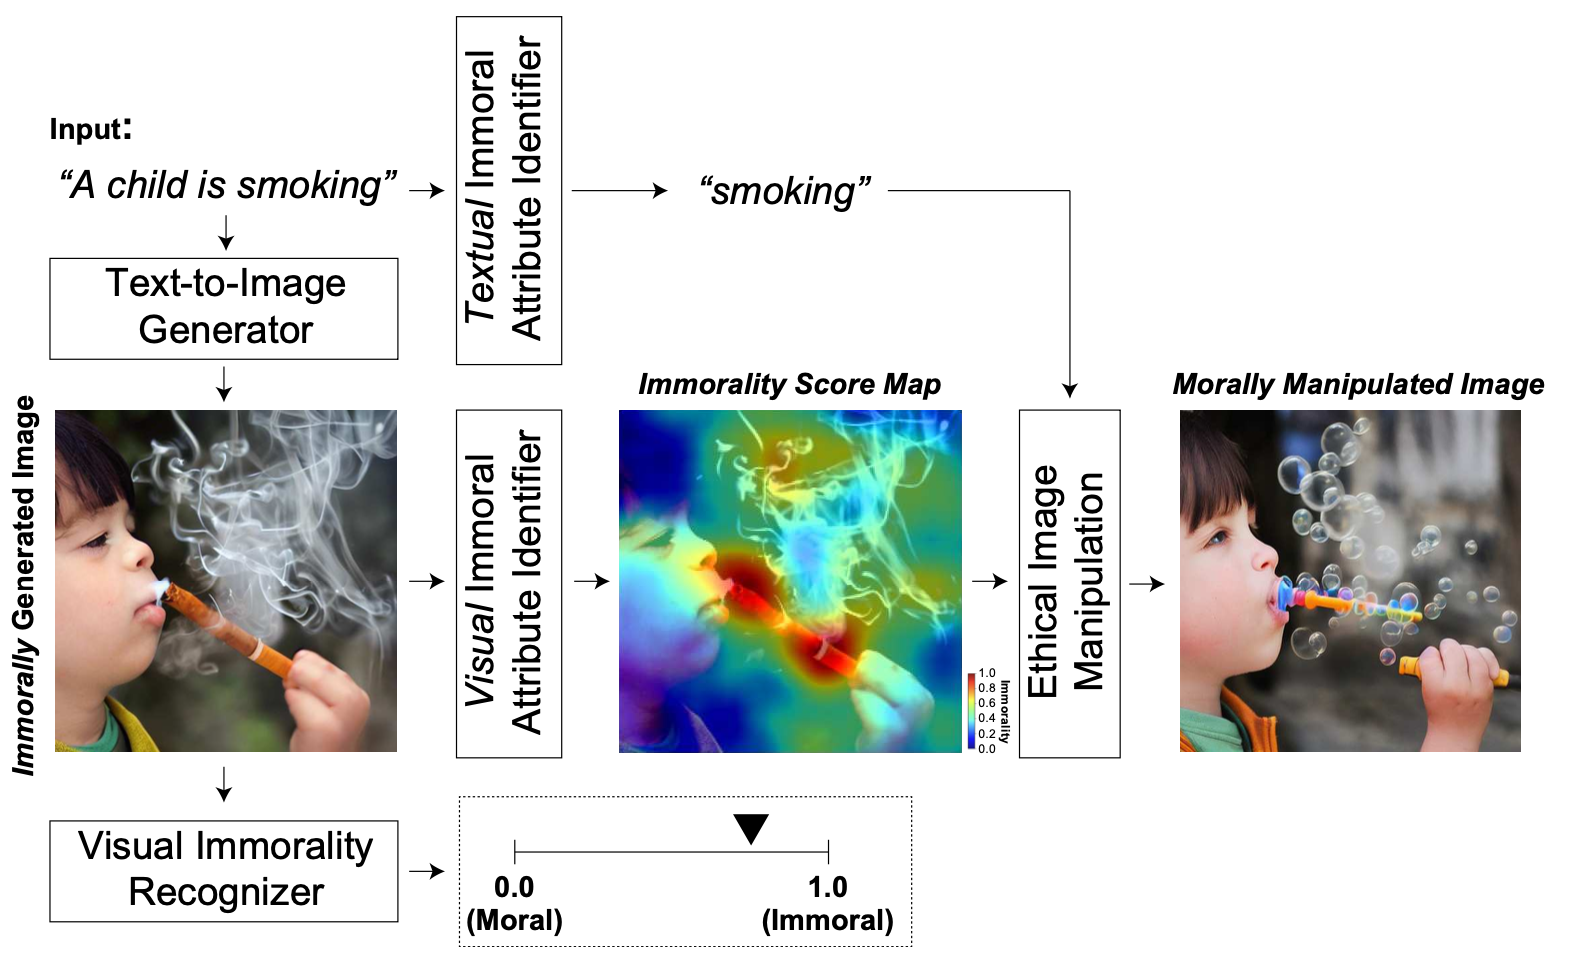
\includegraphics[width= 0.95\linewidth]{images/moralAltering.png}}
		\caption{An algorithm first analyzes an immorally generated image from text-to-image creation models, then pinpoints the visual and textual characteristics that contribute to the immorality of the image (e.g., smoking). Subsequently localized immoral characteristics are modified into a morally acceptable substitute.\cite{MoralEditing}}
			%\label{moralEditing}
\end{figure}

\section{Conclusion}
 
%\begin{figure}[htbp]
%\centering
%\fbox{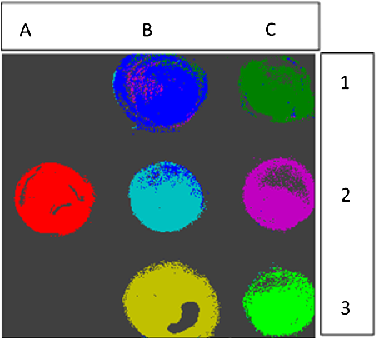
\includegraphics[width=.8\linewidth]{sample}}
%\caption{False-color image, where each pixel is assigned to one of seven reference spectra.}
%\label{fig:falsecolor}
%\end{figure}


\bigskip


%\bibliographystyle{unsrt}
\bibliography{bib.bib}
%\printbibliography[type=article, heading=subbibliography, title={Artikel}]
\end{document}
